% 五号字体,开明式标点处理,不设置默认字体
\documentclass[UTF8,12pt,punct=kaiming,fontset=none]{ctexart}
\usepackage{fontspec}  % 字体
\usepackage{subcaption}  % 节标题
\usepackage[colorlinks=true, linkcolor=magenta, citecolor=magenta, urlcolor=magenta]{hyperref}  % 超链接
\usepackage{geometry}  % 页面布局
\usepackage{fancyhdr}  % 页眉页脚
\usepackage{titlesec}  % 标题
\usepackage{caption}  % 图表标题
\usepackage{floatrow}  % 图表排版
\usepackage{graphicx}  % 图片路径

% 图片路径
\graphicspath{{figures/}}

% 字体
\setCJKmainfont{Source Han Serif SC}
\setCJKsansfont{Source Han Sans SC}
\setmainfont{CMU Serif}

% 布局
\geometry{a4paper,left=2cm,right=2cm,top=2.5cm,bottom=2.5cm}
\setlength{\headheight}{25pt}

% 图表标题
\DeclareCaptionFont{captionfont}{\small}
\captionsetup{font=captionfont}
\floatsetup{style=plaintop}

% 页眉页脚
\pagenumbering{arabic}
\pagestyle{fancy}
\fancyhead[L]{· \hspace{0.1cm} \thepage \hspace{0.1cm} ·}
\fancyhead[C]{红 \hspace{0.1cm} 石 \hspace{0.1cm} 数 \hspace{0.1cm} 电 \hspace{0.1cm} 评 \hspace{0.1cm} 论\\\scriptsize{Review of Redstonic Digital Circuit}}
\fancyhead[R]{第1期\\\scriptsize{2022年2月}}
\fancyfoot[L,C,R]{}

% 首页页码
\input{页码.inc}

% 标题
\title{\vspace{-1.5cm}更高效的乘法器——树状乘法器原理与建造\vspace{-0.5cm}}
\author{@Enity\_303-E3}
\date{}

% 参考文献标注
\newcommand*{\upcite}[1]{
    \textsuperscript{\cite{#1}}
}

\begin{document}
\pdfbookmark{更高效的乘法器——树状乘法器原理与建造}{\thepage}  % 书签
\hypersetup{bookmarksdepth=-1}  % 禁止后续书签
\maketitle
\thispagestyle{fancy}  % 首页页眉页脚
\vspace{-0.7cm}

% 节标题格式
\titleformat{\section}[hang]{\large\sffamily\bfseries}{\textmd{\thesection}}{0.5cm}{}
\titlespacing{\section}{0cm}{0.5ex}{0.2ex}
\setcounter{section}{0}

我们知道,乘法的本质是加法,而加法需要用到全加器,因此这里先单独展示16位全加器\upcite{full_adder}的构造,见图\ref{fig:ordinary-multiplier}(a)。

这里先举个例子,$110\times101$ 可以将乘数$101$ 拆为$1,0,1$,每一位与被乘数$110$相乘,即进行与运算,然后依次向高位移一位,结果分别为11$0,0000,11000$,最后将这些结果加起来,得到最终结果$11110$。一般乘法器就是将这些结果累加起来,得到最终结果。这里也不多赘述一般乘法器的建造过程,只展示整体构造。

由一般乘法器原理容易得到,一个$n$位的乘法器(即最大输入$2^{n-1}\times2^{n-1}$)总共需要$n-1$次加法运算。设全加器计算复杂度为$O(1)$②,若不考虑移位与信号传输延时,则$n$位乘法器计算复杂度为$O(n-1)$。例如,$1111\ 1111\times1111\ 1111$,一般乘法器需要7次加法(即$1111\ 1111+1\ 1111\ 1110+\cdots+111\ 1111\ 1000\ 0000$),如图\ref{fig:ordinary-multiplier}(b)。显然,对于高位(如32或64位)的乘法计算复杂度就很大。

对此,我们可以设计一种更高效的乘法器——树状乘法器。我们不妨先把第1、2位,第3、4位,第5、6位,第7、8位分别相加,这四次加法运算不考虑移位与信号传输延迟是完全可以实现并行的,因此这一轮加法计算复杂度为$O(1)$。同理,将以上结果再两两相加,不断重复只要最后一个结果。不难得出,总体计算复杂度为$O(\log n)$。这就是树状乘法器的原理。而这两两相加的过程,我们能联想到“二叉树”,所以这种乘法器由此得名“树状乘法器”,其结构见图\ref{fig:tree-multiplier-overview}。

这里以8位乘8位为例。如前文提到,乘法器计算$1111\ 1111\times1111\ 1111$的方法为计算$1111\ 1111+1\ 1111\ 1110+\cdots+111\ 1111\ 1000\ 0000$。我们不妨将这8个加数命名为$a_1,a_2,\cdots,a_8$。

\begin{figure}[H]
    \centering
    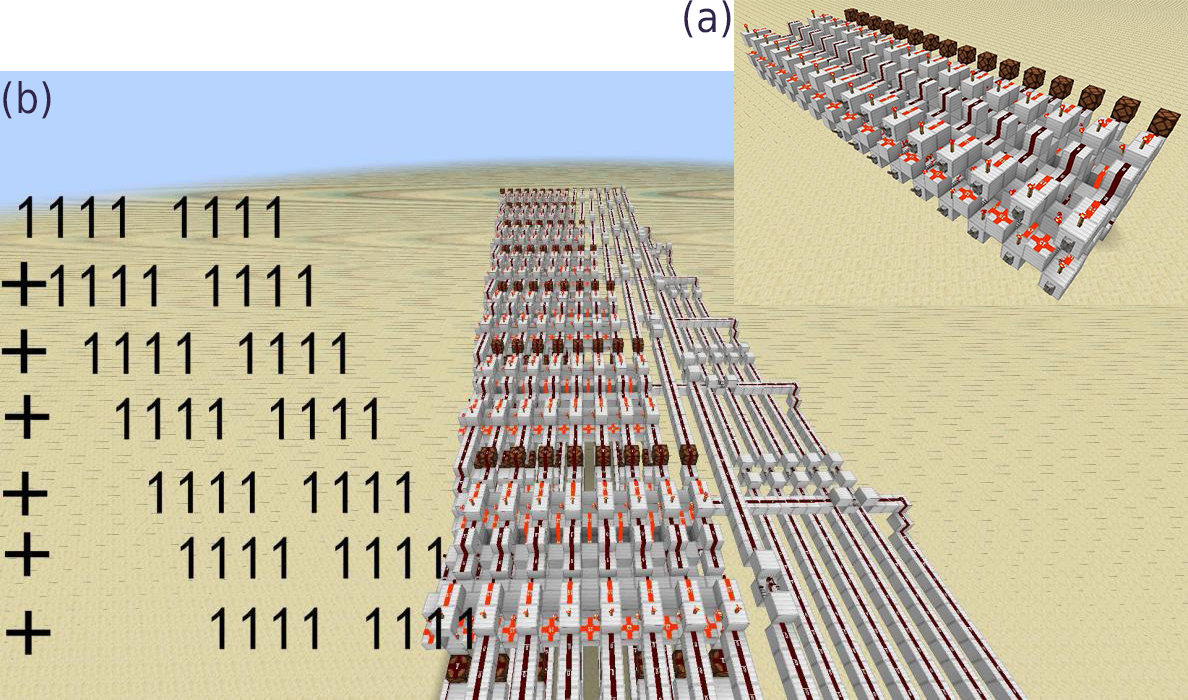
\includegraphics[width=0.85\linewidth]{common_multiplier_example.png}
    \caption{\small (a)单个16位全加器。(b)一般乘法器的结构。}
    \label{fig:ordinary-multiplier}
\end{figure}

第一步:将$a_1$与$a_2$,$a_3$与$a_4$,$a_5$与$a_6$,$a_7$与$a_8$分别使用全加器相加,得到结果分别记为$b_1,b_2,b_3,b_4$,这一步计算复杂度为$O(1)$.

第二步:将$b_1$与$b_2$,$b_3$与$b_4$分别使用全加器相加,得到的结果记为$c_1$和$c_2$,这一步计算复杂度同样为$O(1)$。

第三步:将$c_1$与$c_2$使用全加器相加得到结果$r$,这一步计算复杂度为$O(1)$。$r$是最终的乘法结果。总计算复杂度为$O(\log n)$。因为是8位乘法,故$n=8$。以2为底时,$\log_2n=3$,对应我们所需的三个步骤。

\begin{figure}[h]
    \centering
    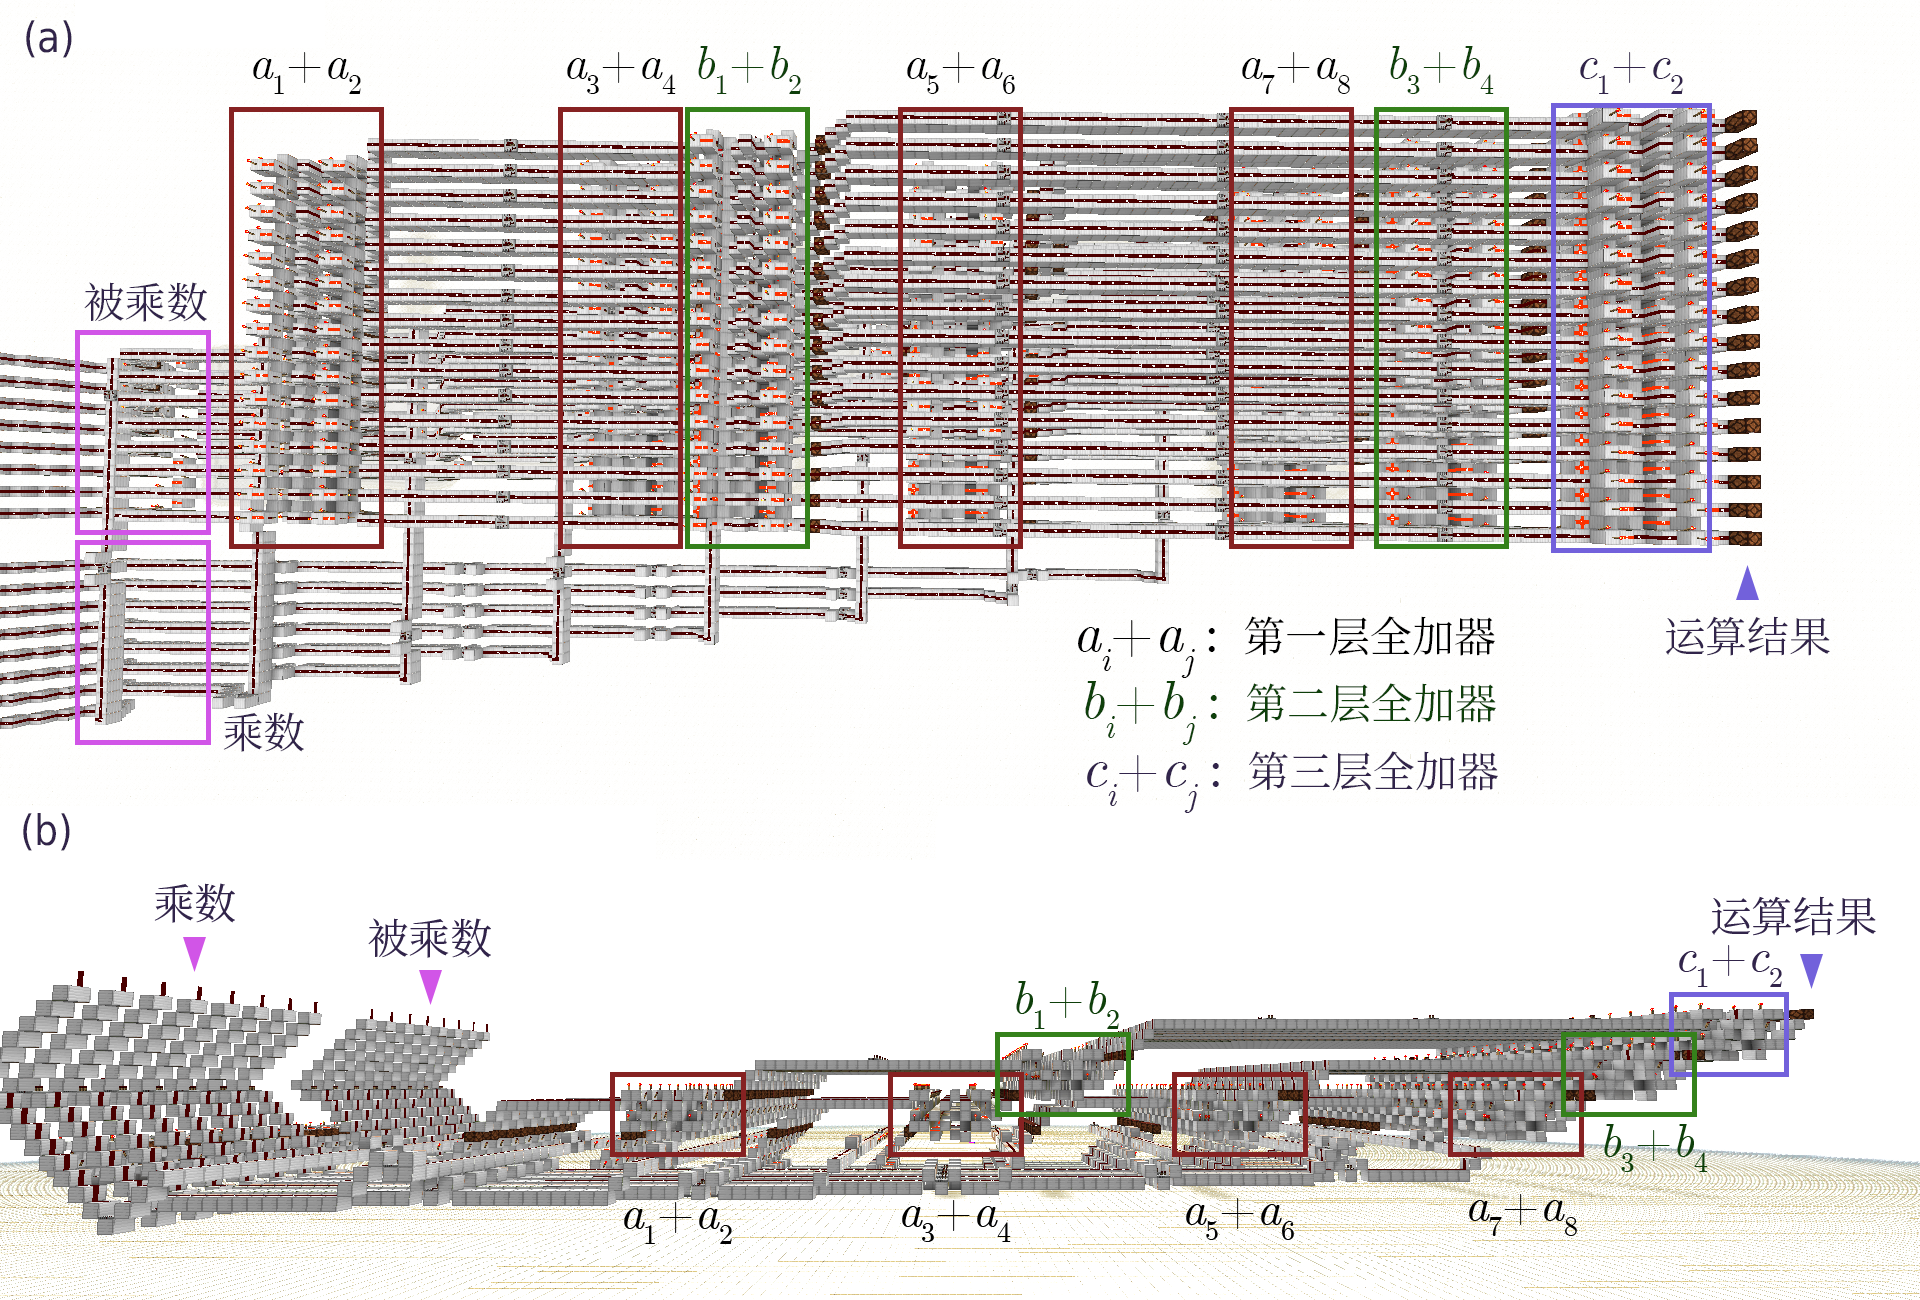
\includegraphics[width=0.97\linewidth]{overview.png}
    \caption{\small 树状乘法器的整体概览,(a)俯视图,(b)侧视图。}
    \label{fig:tree-multiplier-overview}
\end{figure}

树状乘法器有着更低的计算复杂度,并且建造难度较低,此外配合封闭进位加法器(CCA)可以获得更好的效果,这是红石计算器建造中可供选择的方案之一。

最后感谢@辰占鳌头与@mail\_set的提醒与指导。

\bibliographystyle{unsrt}
\bibliography{reference.bib}

\end{document}
